\cotefile{43}
\scanpage{49}
% archive sheet number: 48
\diagram{$\begin{array}{lll}
\displaystyle\prod_{x\in X_0}G(\unsure{\widehat{O}_x|\widehat{\mathcal O}_x}) & & \\
\displaystyle\prod_D\prod_{\substack{x\in |D|\\\mathrm{local}}}G(\widehat{O}_{D,x}) &
\displaystyle\prod_{\substack{\deleted{\unsure{x\in X}}\\D\in X_1}}G(\widehat{O}_D)&\\
&\displaystyle\prod_{\mathrm{local}}G(\unsure{\widehat{K}_D|\widehat{O}_D})&
\end{array}$}

\diagram{\begin{tikzcd}[ampersand replacement=\&,column sep=small]
\displaystyle\prod_x\widehat{\underline{O}}_x^*\arrow[d] \& \& \\
\displaystyle\prod_D\prod_{\substack{x\in|D|\\\mathrm{local}}}\widehat{O}_{D,x}^*\arrow[d]
\&\displaystyle\prod_D\widehat{O}_D^*\arrow[l]\arrow[d]
\&\unsure{O|0|G}\arrow[l,dashed]\arrow[d,dotted,no head]\\
G(K)\big/\displaystyle\prod_x\prod_{\substack{\deleted{\unsure{D\ni x}}\\|D|\ni x}}
(\widehat{O}_{D,x}\otimes_{O_D}K)^*
\&\displaystyle\prod_{\mathrm{local}}\widehat{K}_D^*\arrow[l]
\&K^*\arrow[l]
\end{tikzcd}}

\figure{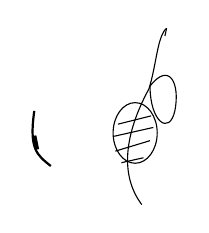
\begin{tikzpicture}[scale=.7]
\draw[line width=.8pt] (-1.6,1.0) .. controls (-1.7,.3) and (-1.55,.2) .. (-1.3,0);
\draw[line width=1.5pt] (-1.6,.55)--(-1.55,.3);
\draw (.35,-.7) .. controls (-.1,-.1) and (.1,.7) .. (.48,1.4) .. controls (.62,1.85) and (.63,2.35) .. (.8,2.5);
\draw (.8,2.5)--(.77,2.36);
\draw (.5,1.45) .. controls (.85,1.9) and (1.05,1.5) .. (.95,1.0) .. controls (.85,.55) and (.5,.8) .. (.5,1.45);
\draw (.23,.6) ellipse (.4 and .55);
\draw (-.08,.76)--(.52,.91) (-.15,.54)--(.56,.7) (-.13,.27)--(.5,.46) (-.02,.06)--(.38,.15);
\end{tikzpicture}}

\figure{\begin{tikzpicture}\draw (0,0) to[bend left=12] (.35,2.5);\end{tikzpicture}}
\diagram{\begin{tikzcd}[ampersand replacement=\&]
-\widehat{\underline O}_x \& O_x\arrow[l]\arrow[d]\\
\unsure{\widehat{\widehat{\underline O}_{x}\otimes_{\underline O_D}\underline O_D}|\widehat{\widehat{\underline O}_{D}\otimes_{\underline O_D}\underline O_{D,x}}} \& O_D\arrow[l]\arrow[d]\\
\&\underline O_{\unsure{\eta|q}}
\end{tikzcd}}

\[
\operatorname{Hom}(K,\coprod_x\deleted{\unsure{I}} I_x)
\]

\diagram{\begin{tikzcd}[ampersand replacement=\&]
K\arrow[r] \& I_D\arrow[r] \& I_x\\
\widehat K_D^* \& \&\widehat O_{D,x}^*
\end{tikzcd}}
\figure{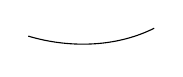
\begin{tikzpicture}\draw (0,.15).. controls (.5,0) and (1.1,0)..(1.6,.25);\end{tikzpicture}}

\figure{\begin{tikzpicture}\draw (0,0)--(.6,3);\end{tikzpicture}}
\diagram{\begin{tikzcd}[ampersand replacement=\&]
\widehat O_D\arrow[d] \& O_D\arrow[l]\arrow[d]\\
\widehat{\underline O}_{D,0} \& O_0\arrow[l]
\end{tikzcd}}

\diagram{\begin{tikzcd}[ampersand replacement=\&,column sep=large]
A_{[p_1>\cdots>p_n]}\&\\
A_{[p_n]}\arrow[u,"{\mathrm{hom\ local}}"]
\&\deleted{\unsure{A_{[p_n]}/p_{n+1}^k A_{[p_{\unsure{n}}]}}}\\
A_{p_n}\arrow[u,"{\mathrm{hom\ local}}"]\arrow[r]
\&A_{p_{n+1}}/p_{n+1}^k A_{p_{n+1}}
\end{tikzcd}}
% The abandoned arrow at the right of A_[p_n] is struck.
\[\deleted{\unsure{\longleftarrow|\longrightarrow}}\]
\diagram{\begin{tikzcd}[ampersand replacement=\&]
\deleted{A_{[p_1]}}\&\\
\deleted{A_{[p_2]}}\arrow[u]\arrow[r]\&\deleted{A_{[p_1]}}
\end{tikzcd}}

\diagram{\begin{tikzcd}[ampersand replacement=\&]
\displaystyle\prod_D\widehat O_D^{\unsure{*|\cdot}}\&\displaystyle\sum\underline O_D\arrow[l]\\
\&K^{\unsure{*|\cdot}}\\
\&O_D
\end{tikzcd}}

\[ A_{[p_1]}\qquad\underline A \]

\diagram{\begin{tikzcd}[ampersand replacement=\&]
\widehat{\underline O}_{D,x}\&\widehat{\underline O}_D\arrow[l]\arrow[d]\&\underline O_D\arrow[l,phantom,"{\unsure{\leftarrow|\twoheadleftarrow}}"]\arrow[d]\\
\deleted{\unsure{*}}\&\widehat K_D\&K^{\unsure{*|\cdot}}\arrow[l]
\end{tikzcd}}

\diagram{\begin{tikzcd}[ampersand replacement=\&]
A_{p_1}\arrow[r]\& A_{\deleted{\unsure{p}}p_2}/p_2^k A_{p_2}
\end{tikzcd}}
\scanpage{50}
% archive sheet number: 49
\unsure{Détermination} des \inserted{hom} $D_p(M)\longrightarrow K_q$ $(q\supset p)$

On peut \unsure{supposer} $A$ local d'idéal \unsure{maximal} $m=q$, $p$ sera un idéal premier quelconque.

\deleted{\unsure{On a|On}} $\operatorname{Hom}(D_p(M),K_q)$ est un \unsure{foncteur} \uline{exact} en $M$, donc de la forme $M\otimes K_{p,q}$, où $K_{p,q}$ est un $A$-module \deleted{\unsure{projectif}} \uuline{plat}, savoir $\operatorname{Hom}(K_p,K_q)$.
% slanted
\margin{\uline{\unsure{covariant}}}

Si $q=p$, on \unsure{obtient} $\widehat A_p=\widehat A_q$.
\scanpage{51}
% archive sheet number: 50
$A$ anneau \unsure{régulier}, de dim finie, \deleted{\unsure{biéquidimensionnel}}

\[
\begin{aligned}
\deleted{D(A)=\coprod_p\underbrace{D_p(A)}_{I_p}}\\
\deleted{DD(A)=\prod_{\unsure{p|qp}}\operatorname{Hom}(I_p,}
\end{aligned}
\]

\[
D(M)=\operatorname{Hom}(M,K_*)=\coprod_p
\underbrace{\operatorname{Hom}(M,\deleted{\unsure{I_p|K_p}}K_p)}_{p\text{-primaire}\quad D_p(M)}
\]
\[
DD(M)=\prod_p\operatorname{Hom}(\deleted{\unsure{D_q(M)|D_p(M)}}D_p(M),K)
\]

\[
D_p(M)=\varinjlim_i U_i
\qquad\text{les $U_i$ sont de longueur finie sur $A_p$.}
\]
\[
\operatorname{Hom}(D_p(M),K)=\varprojlim_i\underbrace{\operatorname{Hom}(U_i,K)}
\]
\[
\operatorname{Hom}\unsure{(}U_i,K_*)=\coprod_q\operatorname{Hom}(U_i,K_q)
\]
\[
\operatorname{Hom}(U_i,K_q)=\varinjlim_j\operatorname{Hom}\unsure{(}U_i,
\underbrace{K_{q,j}}_{\substack{V_j\text{ de longueur}\\\text{finie sur}\\A_q}})
\]

\figure{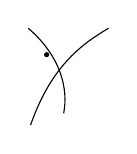
\begin{tikzpicture}[scale=.6]
\draw (-.6,1.2)..controls (.1,.6) and (.25,-.1)..(.15,-.6);
\draw (-.55,-.85)..controls (-.1,.45) and (.6,.9)..(1.1,1.2);
\fill (-.21,.64) circle (.055);
\end{tikzpicture}}

Or $\operatorname{Hom}\unsure{(}U_i,V_j)=0$ si $\unsure{q\not\supset p|q\ne p}$;

donc on aura $\operatorname{Hom}(U_i,K_q)=0$ si $q\not\supset p$,

d'où
\[
\operatorname{Hom}\unsure{(}U_i,K_*)=\coprod_{\underline{\underline q}\supset p}\operatorname{Hom}(U_i,K_q)
\]
\[
\begin{aligned}
DD(M)&=\prod_p\operatorname{Hom}(D_p(M),\coprod_{\underline{\underline q}\supset p}K_q)\\
&=\prod_p\prod_{\underline{\underline q}\deleted{\unsure{\supset}}\unsure{\supset}p}^{\mathrm{local}}\operatorname{Hom}(D_p(M),K_q)
\end{aligned}
\]
\scanpage{52}
% archive sheet number: 51
\diagram{\begin{tikzcd}[ampersand replacement=\&]
\unsure{O|\mathcal O}\&\widehat O_{q_1}\arrow[l]\arrow[d]\arrow[dr,phantom,"\otimes"]\&O_{q_1}\arrow[l]\arrow[d]\\
\&\widehat O_{q_1,q_0}\&O_{q_0}\arrow[l]
\end{tikzcd}}

\figure{\begin{tikzpicture}
\draw (-.7,.35)--(-.45,.8);\fill (-.7,.1) circle (.04);\node[below] at (-.7,.05) {$x$};
\draw (-.25,1.0)..controls (-.05,.3) and (.2,.15)..(.55,-.05);\fill (-.05,.48) circle (.035);
\draw (.05,.95)--(.65,.8);\fill (.85,.86) circle (.035);\fill (1.08,.8) circle (.035);
\draw[line width=1.2pt] (3.3,-.7)--(5,-.7);\foreach \x in {3.3,4.2,5}{\fill (\x,-.7) circle (.065);}
\end{tikzpicture}}

$x$, $\unsure{p|q}$ \unsure{fixés|finis}
\figure{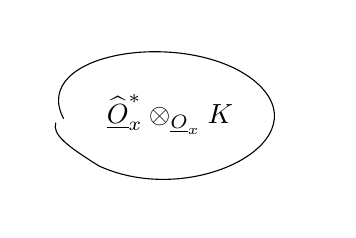
\begin{tikzpicture}
\node at (0,0) {$\widehat{\underline O}_x^{\unsure{*}}\otimes_{\underline O_x}K$};
\draw (-1.35,-.05)..controls (-1.8,.8) and (.2,1.1)..(1.05,.45)..controls (2,-.3) and (.3,-1.2)..(-.9,-.65)..controls (-1.3,-.4) and (-1.5,-.25)..(-1.45,-.1);
\end{tikzpicture}}

\[ A_{[p\supset q]} \]
\diagram{\begin{tikzcd}[ampersand replacement=\&]
A_{[p]}=\widehat A_p\&\\
A_p\arrow[u]\arrow[r]\&A_q/q^n A_q
\end{tikzcd}}
\diagram{\begin{tikzcd}[ampersand replacement=\&]
A_{[p]}=\widehat A_p\&A_p\arrow[l]
\end{tikzcd}}

\[
\begin{aligned}
A_{[p,q]}&=\varprojlim_n\underbrace{A_{[p]}\otimes_A A_q/q^n A_q}\\
&\hspace{3cm}\Vert\\
&\hspace{1cm} A_{[p]}\otimes_{A_p}A_q/q^n A_q\\
&\hspace{3cm}\Vert\\
&\hspace{1cm} A_{[p]}/q^n A_{[p]}\otimes_{\deleted{\unsure{A_q}}A_p} A_q/q^n A_q\\
&\hspace{3cm}\Vert\\
&\hspace{1cm}\deleted{\unsure{(A/q^n A}}\\
&\hspace{1cm} A_{[p]}/q^n A_{[p]}\otimes_{A_p} A_q\\
&\hspace{3cm}\Vert\\
&\hspace{1cm}\underbrace{A_{[p]}/q^n A_{[p]}}\otimes_A A_q\\
&\hspace{3cm}\Vert\\
&\hspace{1cm}\deleted{\unsure{A_p}(A/q^n A)_{[p]}}
\end{aligned}
\]
\margin{On peut y \unsure{remplacer} $q^n$ par $q^{(n)}$}
\margin{\unsure{anneau} \unsure{semi local}, \unsure{non complet}, \unsure{mais quotient} \unsure{d'un complété} \unsure{localisé} de $\widehat{A_p/q A_p}\otimes_{A_p/q A_p}\unsure{1|L}$}
\diagram{\begin{tikzcd}[ampersand replacement=\&]
\widehat{A_p/q^n A_p}=(A/q^n A)_{[p]}\&{}\arrow[l]
\end{tikzcd}}

\figure{\begin{tikzpicture}[scale=.5]
\draw (0,4.6) to[out=-80,in=10] (-2.4,2.5) to[out=190,in=70] (-2.8,1.6) to[out=250,in=20] (-4.2,.4) to[out=200,in=60] (-5,-.6);
\draw (6.5,5) to[out=-65,in=65] (7,-.8);
\end{tikzpicture}}
\scanpage{53}
% archive sheet number: 52
\diagram{\begin{tikzcd}[ampersand replacement=\&]
p'\&\deleted{\unsure{p'}}q'\\
p\arrow[r,no head,"{\deleted{\unsure{*}}}"]\arrow[r,bend right=25,no head]\&\deleted{\unsure{m}}q
\end{tikzcd}}
\[\unsure{\operatorname{Hom}}(K_p,K_m)\unsure{=|:}A_{mp}\]

\figure{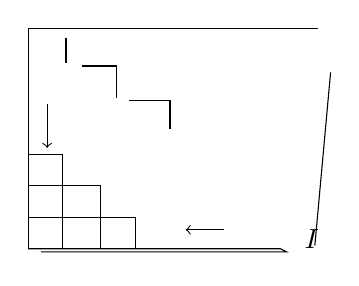
\begin{tikzpicture}[scale=.8]
\draw (0,0)--(0,3.5)--(4.6,3.5);
\draw (4.8,2.8)--(4.55,.05);
\draw (0,0)--(4,0)--(4.1,-.05)--(.2,-.05);
\draw (0,0) rectangle (.55,.5);\draw (0,.5) rectangle (.55,1);\draw (0,1) rectangle (.55,1.5);
\draw (.55,0) rectangle (1.15,.5);\draw (.55,.5) rectangle (1.15,1);\draw (1.15,0) rectangle (1.7,.5);
\draw (.6,3.35)--(.6,2.95) (.85,2.9)--(1.4,2.9)--(1.4,2.4) (1.6,2.35)--(2.25,2.35)--(2.25,1.9);
\draw[->] (.3,2.3)--(.3,1.6);\draw[->] (3.1,.3)--(2.5,.3);
\node at (4.5,.15) {$I$};
\end{tikzpicture}}

\[p\subset p'\qquad q'\subset q=m\qquad A_m/p^n A_m=B\]
\diagram{\begin{tikzcd}[ampersand replacement=\&]
A_{q,p''}\arrow[d]\&\&\\
A_{\deleted{\unsure{p}}q,p'}\arrow[d]\&A_{q',p'}\arrow[l]\arrow[d]\&\\
A_{\deleted{\unsure{p}}q,p}\&A_{q',p}\arrow[l]\&A_{q'',p}\arrow[l]
\end{tikzcd}}
\diagram{\begin{tikzcd}[ampersand replacement=\&]
\&p'\arrow[dr,no head,"\subset"]\&\\
p\arrow[ur,no head,"{\unsure{\subsetneq|\ne}}"]\arrow[dr,no head,"\subset"']\&\&q\\
\&q'\arrow[ur,no head,"\subsetneq"']\&
\end{tikzcd}}

\[\operatorname{Hom}(K_p,K_q)\]
\diagram{\begin{tikzcd}[ampersand replacement=\&]
\&\&p''\arrow[ddr,no head,"\subset"]\&\\
\&p'\arrow[ur,no head,"\subsetneq"]\&\&\\
p\arrow[r,no head,"\subsetneq"]\arrow[ur,no head,"\subsetneq"]\arrow[ddrr,no head,"\subset"']\&p'\arrow[r,no head,"\subseteq"]\&q'\arrow[r,no head,"\subsetneq"]\&q\\
\&\&\&q'\arrow[u,no head,"\subsetneq"']\\
\&\&q''\arrow[ur,no head,"\subsetneq"']\&
\end{tikzcd}}
\[\underset{\longleftrightarrow}{\operatorname{Hom}(K_*,K_*)}\]
\[
A_{q,p}=(\coprod_{p'}A_{q,p'})\unsure{\amalg|\coprod}(\coprod_{q'}A_{q',p})\big/
\]

$I$ ensemble ordonné, tel que

(i) deux \unsure{objets} $\deleted{\unsure{p,q}}\inserted{x,y}$ tels que $\deleted{p\leq}\,x<y$ \unsure{peuvent|peut} être \unsure{joints|joint} par une chaine saturée

(ii) Deux chaines saturées ont $=$ longueur

\deleted{Si $x,y$} On \unsure{suppose définis} $A_{x,y}\in\unsure{\mathcal C|\mathcal E}$ si $\left\{\begin{aligned}&\deleted{\unsure{d(x,y)}}x\leq y\\&\text{et }d(x,y)\leq1\end{aligned}\right.$

On va en construire un \deleted{\unsure{complexe, bicomplexe}} \unsure{objet} à une \unsure{``puissance''} \unsure{de $I$ indexée},
\scanpage{54}
% archive sheet number: 53
\[
\begin{aligned}
A_{[p,q]}&=\varprojlim A_{[p]}\otimes_{A_p}A_q/q^n A_q\\
&=\varprojlim A_{[p]}/q^n A_{[\unsure{p}]}\otimes_{A_p}A_q/q^n A_q
\end{aligned}
\]
\[A_{[p,q,\unsure{r|v|\varpi}]}\qquad\text{etc}\]

$X$ \uline{ensemble ordonné}

$S_X$ ensemble simplicial associé, dont les $n$-simplexes sont les chaines
\[
\begin{aligned}
x_0\leq x_1\leq\cdots\leq x_n\\
\longleftarrow
\end{aligned}
\]
[i.e. les applications croissantes de $[0,n]=\underline\Delta_n$ dans $X$]

À tout $\sigma\in S_X$ est associé un $A_\sigma$

À tout \unsure{opérateur|opération} \deleted{face} \inserted{\unsure{simplicial}} $u:\underline\Delta_m\longrightarrow\underline\Delta_n$ (\uline{croissant}) est associé un hom
\diagram{\begin{tikzcd}[ampersand replacement=\&]
\deleted{A_\sigma}\&S_X^n\arrow[r,"u^*"]\&S_X^m
\end{tikzcd}}

et si $\sigma\in S_X^{\unsure{n|m}}$, d'où $u^*(\sigma)\in S_X^m$, on a un \unsure{morphisme}
\[
\varphi(\sigma,u):\quad A_\sigma\longleftarrow A_{u^*\sigma},
\]
De façon \unsure{fonctorielle}.
\scanpage{55}
% archive sheet number: 54
Ainsi, les $A_\sigma$ forment un \uline{faisceau} sur l'ensemble simplicial $S_X$. \deleted{\unsure{On l'appelle} un \uline{faisceau \unsure{étagé}}} [On peut dire qu'on a un objet simplicial dans la catégorie des ensembles \deleted{\unsure{linéaires et anneaux|locaux et anneaux}} \inserted{\unsure{annelés}}]

\deleted{\unsure{sup} \unsure{fibré en} \illegible{3}}
\inserted{Ici, \unsure{tous|tous les} hom de \unsure{dégénérescence|dégénérescences} sont \unsure{des} \uline{isomorphismes}, pour les coefficients [\unsure{on a aussi} \unsure{un homomorphisme des} \unsure{simplexes non dégénérés}]}

Dans le \unsure{cas|propos} actuel, il y a lieu de \uline{négliger} tout ce qui provient des simplexes de la forme \deleted{$\unsure{\partial_i\partial_j\sigma}$, \unsure{où}} \deleted{\unsure{un simplexe non} \uline{\unsure{dégénéré}}} \deleted{[i.e. des chaines} $\partial_i\sigma$, où $\partial_i$ est un opérateur face qui n'est pas un opérateur ``de coin'', $\sigma$ \uline{\unsure{non|un}} \uline{\unsure{épuisé|épuré}} [\unsure{Cela|Ceci} revient à ne retenir que les chaines saturées \deleted{\unsure{\sigma}}, et \deleted{\unsure{parmi elles}} \unsure{des|dont}

\figure{\begin{tikzpicture}[x=1cm,y=.7cm]
\draw[gray] (0,3)--(4,3);\draw[line width=1.5pt] (0,2.9)--(0,3.1) (2,2.9)--(2,3.1) (4,2.9)--(4,3.1);
\draw[gray] (.15,2.93)..controls (.9,2.65) and (1.15,3.15)..(1.55,3.08)..controls (1.8,3.35) and (1.95,3.3)..(2,3.05);
\draw (1.94,3.55)--(2,3.48)--(2.06,3.55);\draw (1.94,3.28)--(2,3.20)--(2.06,3.28);\draw (1.94,2.9)--(2.06,3.1) (1.94,3.1)--(2.06,2.9);
\draw[gray] (0,2)--(4,2);\draw[line width=1.5pt] (0,1.86)--(0,2.14) (3.5,1.86)--(3.5,2.14);\draw (4,1.92)--(4,2.06);
\draw[gray] (1,1)--(5.5,1);\foreach \x in {1,1.6,2.2,2.8,3.4,4,4.6,5.5}{\draw[gray] (\x,.96)--(\x,1.15);}
\draw[gray] (1,-.4)--(6,-.4);\fill (1,-.4) circle (.035);\draw (1,-.5)--(1,-.18);\draw (6,-.4) circle (.035);
\end{tikzpicture}}
\diagram{\begin{tikzcd}[ampersand replacement=\&]
(x_0-\,-x_n)\arrow[d]\\{}\arrow[d]\\
(x_0-\widehat x_p-x_n)\\
x_0\quad x_1\quad x_n\\
x_0-x_n
\end{tikzcd}}

\unsure{on peut en faisant intervenir encore des} \unsure{isomorphismes}).
\scanpage{56}
% archive sheet number: 55
\margin{[\unsure{Sous rés.|Sans rés.} des questions de dégénérescences)}
$K^*$ \deleted{\unsure{complexe}} objet cosimplicial dans une catégorie abélienne $\unsure{\mathcal C|C}$

C'est donc un \deleted{objet} $\mathcal C$-module gradué sur l'anneau gradué $S$ engendré par les $\partial_i^n$, \deleted{$\unsure{s_i^n|\sigma_i^n}$} \inserted{$(0\leq i\leq n+1)$} avec les relations qu'on sait. \deleted{\unsure{On va}} On va y introduire les \uline{relations}
\[
\partial_i^n=0\qquad\text{pour}\quad1\leq i\leq n
\]
\margin{$\partial_i^n:\Delta^n\longrightarrow\Delta^{n+1}$\par $0\leq i\leq n+1$}

\unsure{donc considérons|en considérant} dans chaque $K^n$ le sous-objet somme des $K^i\longrightarrow K^n$, où \deleted{$K^i$} $i<n$ et où
\[
\deleted{\left\{\begin{aligned}
&\partial_i^n K^{n-1}&&1\leq i\leq n\\
&\unsure{u_2|u}\partial_i^{n-1}K^{n-2}&&1\leq i\leq n\\
&\text{--}\\
&u\quad K^0
\end{aligned}\right.}
\]
$K^i\longrightarrow K^n$ est une opération simpliciale qui correspond à une application \unsure{strictement} croissante de $\underline\Delta^i$ dans $\underline\Delta^n$ qui \uline{n'est pas d'un \unsure{seul} tenant}. On \unsure{trouve|forme} un $K'^n\subset K^n$, et évidemment on a ainsi un \uline{co-\deleted{\unsure{complexe}}objet simplicial} \inserted{$K'^*$} de $K^*$

\diagram{\begin{tikzcd}[ampersand replacement=\&]
\deleted{\overset{\bullet}{x_0}\leq x_1\quad\unsure{x_{n-1}}\leq\overset{\bullet}{x_n}}\arrow[r,no head]\&\\
(x_0,x_1,x_{\unsure{n|2}})\arrow[d]\&\\
(x_0,x_{\unsure{2|n}})\&
\end{tikzcd}}
\diagram{\begin{tikzcd}[ampersand replacement=\&]
A_{(x_0x_1x_2)}\\
A_{[x_0,x_2]}\arrow[u]
\end{tikzcd}}
\figure{\begin{tikzpicture}\draw (0,.15) to[out=-15,in=200] (2.6,.8) to[out=20,in=180] (3.1,.85);\end{tikzpicture}}
\diagram{\begin{tikzcd}[ampersand replacement=\&,column sep=large]
\&\displaystyle\sum A_{[x_0,x_1,x_2]}\&\&\\
\displaystyle\sum A_{[x_0,x_1]}\&\displaystyle\sum A_{[x_1,x_2]}\& A_{[x_0,x_2]}\arrow[ul]\&\\
\underline{A_{[x_0]}}\arrow[u]\arrow[rrr,bend right=45]\&\underline{A_{[x_1]}}\arrow[ul]\arrow[u]\&\underline{A_{[x_2]}}\arrow[u]\&{}
\end{tikzcd}}
\figure{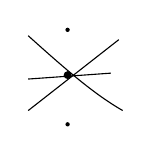
\begin{tikzpicture}[scale=.5]
\draw (-1,1)..controls (0,.1) and (.7,-.5)..(1.4,-.9);\draw (-1,-.9)--(1.3,.9);\draw (-1,-.1)--(1.1,.05);
\fill (0,0) circle (.1);\fill (0,1.15) circle (.055);\fill (0,-1.25) circle (.055);
\end{tikzpicture}}

\[A_{[x_0\quad x_1}\]
\[x_0,x_2\]
\[A_{[x_0,x_2]}\qquad\partial_1^1 A_{[x_0,x_2]}\]
\diagram{\begin{tikzcd}[ampersand replacement=\&]
\unsure{0|o}\&K''\arrow[l]\arrow[r,no head]\&K'\arrow[r,no head]\&K\arrow[r]\&0
\end{tikzcd}}

\figure{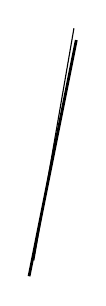
\begin{tikzpicture}\draw[line width=1pt] (0,0)--(.6,3);\draw (.06,.2)--(.57,3.15);\end{tikzpicture}}
\scanpage{57}
% archive sheet number: 56
\[-\]
\diagram{\begin{tikzcd}[ampersand replacement=\&,column sep=large]
A_{[x_1,x_2\deleted{\unsure{]}},-x_n]}\arrow[r]
\&\displaystyle\prod_{\substack{\unsure{x_0}\unsure{,}\\\text{\unsure{précède|précéde}}\\x_1}} A_{[x_0,x_1,-x_n]}\arrow[l,bend left=25,"d_0^{n-1}"']\arrow[r,"d_0^n"']
\&\displaystyle\prod_{\substack{x'_0\unsure{\ne|<}x_0\\(x'_0\ \text{préc.}\ x_0\ \text{\unsure{strict}})}} A_{[x'_0,x_0,x_1,-x_n]}
\end{tikzcd}}

\figure{\begin{tikzpicture}[scale=.7]
\draw[line width=.9pt] (-4,1)--(-1, .8);\draw (-4,.9)--(-4,1.1) (-3.2,.88)--(-3.2,1.08) (-1,.68)--(-1,.91);
\draw (-.4,1.5)--(5,1.5);
\node at (2,0) {$\left\{\begin{aligned}d'^2&=0\\d''^2&=0\\d'd''&=d''d'\end{aligned}\right.$};
\draw (2.5,1.9)..controls (0,2.2) and (-1,-.7)..(1,-1.5)..controls (4,-2.6) and (5,1.4)..(2.7,2);
\fill (4.15,.8) circle (.055);
\draw (3.6,.75)..controls (4.1,1.15) and (4.3,.65)..(3.6,.75);
\draw (4,.65)..controls (4.7,.9) and (4.25,-.25)..(5,-.7)..controls (4.3,-.55) and (3.8,-.65)..(4,-1)..controls (3.1,-.7) and (3.5,-1.2)..(3.65,-1.35);
\end{tikzpicture}}

\diagram{\begin{tikzcd}[ampersand replacement=\&]
A_{[x_0,x_n]}\arrow[r]\&\displaystyle\prod\deleted{\unsure{A_{[x_0x_1x_n]}}}\quad\displaystyle\prod A_{[x_0x_{\unsure{i|1}}x_n]}
\end{tikzcd}}
\diagram{\begin{tikzcd}[ampersand replacement=\&,column sep=small]
\&A_{[x_0x_{n-1}]}\arrow[dl]\arrow[dr]\&\&\&A_{[x_1,x_n]}\arrow[dl]\arrow[dr]\&\\
A_{[x_0,x_{n-1},x_n]}\&\&{}\&A_{[x_0,x_1,x_n]}\&\&{}
\end{tikzcd}}
\[\begin{array}{c|c}x_0&x_n\\\mathrm{min}&\text{\unsure{maximal|max}}\end{array}\]
\unsure{non inversibles|non réversibles}

\[X\qquad\prod\unsure{\widehat{\underline O}_x|\widehat{\underline{\mathcal O}}_x}\]
\[C\qquad\prod_{\mathrm{loc}}\widehat K_x\qquad K\]
\[\cdot\]
\diagram{\begin{tikzcd}[ampersand replacement=\&]
\displaystyle\prod G(\underline O_x)\arrow[d]\&\unsure{0|O}\arrow[l]\arrow[d]\\
\displaystyle\prod_{\mathrm{loc}}G(\unsure{\widehat K_x|\widehat U_x})\&\unsure{G(M)|G(K)}\arrow[l]
\end{tikzcd}}
\diagram{\begin{tikzcd}[ampersand replacement=\&]
G(\widehat A)\arrow[d]\&\\
G(\unsure{\widehat K})\&G(M)\arrow[l]
\end{tikzcd}}
\[H\]
\diagram{\begin{tikzcd}[ampersand replacement=\&]K\arrow[r]\&K/A\end{tikzcd}}
\[G(K)\qquad G(K)/G(A)\]

\figure{\begin{tikzpicture}[x=.7cm,y=.7cm]
\draw (0,2.4)--(3.7,2.2) to[out=0,in=130] (5.4,.7) to[out=-30,in=180] (8.5,0);
\end{tikzpicture}}
\scanpage{58}
% archive sheet number: 57
\diagram{\begin{tikzcd}[ampersand replacement=\&,column sep=tiny,row sep=large]
\&A_{[x_0x_1x_2x_3]}\&\&\&\&\&\&\\
A_{[x_0x_1x_2]}\arrow[ur]\&A_{[x_1x_2x_3]}\arrow[u]\&\deleted{\unsure{A_{[x_2x_3x_n]}}}\&A_{[x_0x_2x_3]}\arrow[ull]\&A_{[x_0x_1x_3]}\arrow[ulll]\&\&\&\\
A_{[x_0x_1]}\arrow[u]\&A_{[x_1x_2]}\arrow[ul]\arrow[u]\&A_{[x_2x_3]}\arrow[ul]\&\deleted{\unsure{A_{[x_1x_3]}}}\&A_{[x_0x_2]}\arrow[ul]\&A_{[x_0x_3]}\arrow[ull]\arrow[ulllll]\&\deleted{\unsure{A_{[x_0x_3]}}}\arrow[ulllll]\&A_{[x_1x_3]}\arrow[ulll]\\
A_{[x_0]}\arrow[u]\&A_{[x_1]}\arrow[ul]\arrow[u]\&A_{[x_2]}\arrow[ul]\arrow[u]\&A_{[x_3]}\arrow[ul]\&\&\&\&
\end{tikzcd}}
\[\deleted{\unsure{A_{[x_1x_3]}}\quad\unsure{A_{[x_1x_3]}}}\]

\[
\unsure{\overline{A_{[x_0x_2x_3]}}\cap
\frac{\overline{A_{[x_0x_1x_3]}}}{\overline{A_{[x_0,x_3]}}}
|\frac{\overline{A_{[x_0x_2x_3]}}\cap\overline{A_{[x_0x_1x_3]}}}{\overline{A_{[x_0,x_3]}}}}
\]
\diagram{\begin{tikzcd}[ampersand replacement=\&,column sep=small,row sep=large]
0\&\&(A_{[x_0x_2x_3]}+A_{[x_0x_1x_3]})\&\&\\
\&A_{[x_0x_2]}\unsure{*|\times}\arrow[ur]\&A_{[x_1,x_3]}\times\arrow[u]\&A_{[x_0x_2x_3]}\times\arrow[ul]\arrow[r,no head,bend left=40,start anchor=west,end anchor=east]\arrow[r,no head,bend right=40,start anchor=west,end anchor=east]\&A_{[x_0x_1x_3]}\arrow[ull]\arrow[dd,bend left=45]\\
0\&A_{[x_0x_2]}\arrow[u]\arrow[urr]\&A_{[x_0x_3]}\arrow[ur]\arrow[urr]\&A_{[x_1x_3]}\arrow[ul]\arrow[ur]\&\\
\&\&\&\&\operatorname{Im}A_{[x_0x_2]}+\operatorname{Im}A_{[x_1x_3]}
\end{tikzcd}}
\diagram{\begin{tikzcd}[ampersand replacement=\&]
\unsure{K_0|S_0}\&S_1\&S_2\&S_{n-1}\&S_n\arrow[l,"d_i^n"]\arrow[d]\\
\&\&\&d_i^n\sigma\&\sigma\\
\&\&\&A_{d_i^n\sigma}\&A_\sigma
\end{tikzcd}}
\[\begin{array}{cccc}\alpha&\beta&-\overline\alpha&-\overline\beta\\\alpha&&\unsure{\circ.|0.}&\beta\end{array}\]
\noindent\rule{\linewidth}{.3pt}

\[K\qquad d_i^n\qquad0\leq i\leq n+1\qquad d'\pm d''\]
\[
\bigcap_{1\leq i\leq n+1}\operatorname{Ker}d_i^n\qquad
\unsure{\bigcap|\coprod}_{\underline{1\leq i\leq n}}\operatorname{Coker}d_i^n
\]
\[d_i^{n+1}d_0^n x=0\]
si $1\leq i\leq n+2$

\figure{\begin{tikzpicture}[x=.7cm,y=.6cm]
\draw (0,4)--(4,4);\draw[line width=1.4pt] (1.2,4)--(4,4);\foreach \x in {0,1.2,4}{\draw (\x,3.85)--(\x,4.15);}
\draw (-1,3)--(3.5,3);\draw[line width=.8pt] (0,3)..controls (1,2.9) and (2,2.9)..(2.6,3);\foreach \x in {-1,0,2.6,3.5}{\draw (\x,2.85)--(\x,3.15);}
\draw (-4,1)--(-2,1);\draw[line width=1.2pt] (-4,1)--(-2,1);\foreach \x in {-4,-2}{\draw (\x,.85)--(\x,1.15);}
\node[below] at (-3,.8) {$\Delta^n$};
\draw (-1.3,1)--(5,1);\draw[line width=1.2pt] (.6,1)--(2.1,1);\foreach \x in {-1.3,.6,2.1,5}{\draw (\x,.88)--(\x,1.12);}
\node[below] at (.5,.8) {$\Delta^{n+1}$};\node[below] at (4,.8) {$\Delta^{n+2}$};
\draw (-6,-1)--(-5.2,-1);\draw (-4.8,-1)--(-2.3,-1);\foreach \x in {-6,-5.2,-4.8,-2.3}{\draw (\x,-1.1)--(\x,-.9);}
\end{tikzpicture}}
\diagram{\begin{tikzcd}[ampersand replacement=\&]
A_{[x_0,x_2]}\&A_{(x_0,x_0,x_2]}\arrow[l]\\
\&\deleted{\unsure{d|\partial|a}}
\end{tikzcd}}
\[x_0\quad x_1\quad\underbrace{x_{\unsure{2|i|1|n}}-x_n}\]
\[\cdot\quad\cdot\quad\cdot\]
$1^\circ)$ $\bigcap$\uline{Ker des dégénérescences}
\scanpage{59}
% archive sheet number: 58
\[\begin{array}{c} \unsure{rg}\quad q\\\unsure{rg}\\p\end{array}\]
\diagram{\begin{tikzpicture}[scale=.72,transform shape]
\node[inner sep=0] (matrix) {$\begin{array}{c|c|c|c}
{}&\text{\unsure{max.}}&\text{\unsure{ht. 1}}&0\\\hline
\text{\unsure{max.}}&\begin{gathered}\widehat A\\\downarrow\end{gathered}&0&0\\\hline
\unsure{1}&\begin{gathered}\displaystyle\varprojlim\underbrace{\widehat A/\unsure{\varpi|\pi}^n\widehat A\otimes_A A_\varpi/\varpi^n A_\varpi}_{\widehat A\otimes_A A_\varpi/\varpi^n A_\varpi}\\A_{[m,\varpi]}\\\downarrow\end{gathered}&\begin{gathered}\longleftarrow\widehat A_\varpi\\\downarrow\end{gathered}&0\\\hline
0&\displaystyle\prod_\varpi A_{[m,\varpi,0]}&\begin{gathered}\longleftarrow\widehat A_\varpi\otimes_A K=\widehat K_\varpi\\A_{[\varpi,0]}\end{gathered}&\longleftarrow K\\\hline
\end{array}$};
\draw ([yshift=-.3cm]matrix.south west) to[out=10,in=210] ([yshift=-1.2cm]matrix.north east);
\end{tikzpicture}}
% The diagonal stroke is reproduced across the table; guide/cancellation status remains uncertain.
\[m>\varpi>0\]

\[S_A(\unsure{M|A})\]
\[\operatorname{Hom}_A(M,\unsure{\mathcal A|A})\]
\diagram{\begin{tikzcd}[ampersand replacement=\&]
\operatorname{Ext}^*(M,A)\\
H^*\operatorname{Ext}^*(M,\mathcal A)\arrow[u,Rightarrow]
\end{tikzcd}}
\[\operatorname{Ext}^*(\widehat M,A)\qquad\widehat A\quad\widehat K\quad K\]

\[\underbrace{\operatorname{Hom}(M,A),\ \operatorname{Ext}^1(M,A)}\ -\]
\diagram{$\begin{array}{c|c|c}
\begin{gathered}\widehat A^*\\\downarrow\end{gathered}&1&1\\\hline
\begin{gathered}\displaystyle\varprojlim(\widehat A\otimes_A A_\varpi/\varpi^n A_\varpi)^*\\\downarrow\end{gathered}&\begin{gathered}\longleftarrow\widehat A_\varpi^*\\\downarrow\end{gathered}&\\\hline
{}&\longleftarrow\widehat K_\varpi^*&\longleftarrow K^*\\\hline
\end{array}$}

\[
\begin{aligned}
\operatorname{Hom}(K_p,K_q)&=A_{q,p}\\
&(q\supset p
\end{aligned}
\]
$A$ \unsure{anneau local}
\diagram{\begin{tikzcd}[ampersand replacement=\&]
0\arrow[r]\&A\arrow[r]\&\unsure{\mathcal A_0|A_0}\arrow[r,no head]\&\unsure{\mathcal A_1|A_1}\arrow[r]\&0
\end{tikzcd}}
\[
\text{\uuline{$\operatorname{Ext}^1(M,A)$}}-\boxed{\begin{gathered}\unsure{p|\rho},\ \unsure{p|\rho}\\
\operatorname{Ext}^{\unsure{p}}(\unsure{\widehat M},\unsure{\widehat A})\longrightarrow
\unsure{K^{p+}\operatorname{Ext}^p(M,A)}
\end{gathered}}
\]

\figure{\begin{tikzpicture}\draw (0,.7) to[out=-90,in=0] (-.7,0);\draw (0,0)--(1,-1);\end{tikzpicture}}
\scanpage{60}
% archive sheet number: 59
\margin{[\unsure{dans ce cas} \deleted{\unsure{les objets} $(x,\unsure{\zeta|\xi})$ \unsure{de $A_c$}} \inserted{$X$ est une catégorie, \unsure{définie par les|désignons par les}} \unsure{morphismes de} $X$: \unsure{les couples} $(c,\zeta)$, où \unsure{$c$ est une chaine saturée de $x_0$ à $x_n$} et $\zeta\in A_c$]}
\unsure{est|une} \uline{associative}. L'étendant par $0$ si \deleted{$\unsure{A_c}$ et} $\unsure{c'|c}$ et $c$ ne sont pas composables, la somme des $A_c$ devient un anneau $A^*$ [en général non commutatif], \inserted{\uline{gradué} par la longueur des chaines}, la somme des $A_x$ \unsure{devient|donne} un sous-anneau (commutatif), \unsure{soit|savoir} $A^0$.

$A^1$ est la somme des $A_{[x_0,x_1]}$, soit $\Theta$ l'élém de $A^1$ dont les composantes sont $1_{[x_0,x_1]}$.

\deleted{Quel est $\Theta^2$ ?} On a
\[
\Theta^2=\sum_{\substack{(x_0,x_1)\\(\unsure{x_0|y_0},y_1)\\\text{chaines}\\\text{saturées}}}
1_{[x_0,x_1]}\cdot1_{[y_0,y_1]}
=\sum_{\substack{[x_0,x_1,x_2]\\\text{chaines}\\\text{saturées}}}\cdot1_{[x_0,x_1,x_2]}
\]

On va maintenant diviser par l'idéal \inserted{bilatère} engendré par $\Theta^2$, \deleted{[\unsure{ce qui signifie aussi}, \unsure{semble-t-il}, \unsure{que l'on impose que}}

\uline{$\unsure{u_1+\partial u_2}$}
En dim $0$ et $1$, cela ne tue rien, en dim $2$ il faut \unsure{coégaler} les
\[
\sum_{\substack{x_1\\\text{\unsure{intermédiaire} à}\\a\ \text{et}\ b\\(\text{\unsure{où}}\ \delta(a,b)=2)}}\varphi
\]

\figure{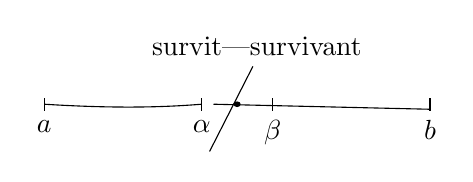
\begin{tikzpicture}[x=1cm,y=.8cm]
\draw (0,0)..controls (.9,-.07) and (1.5,-.05)..(2,0);\draw (2.15,0)--(4.9,-.08);
\foreach \x in {0,2,2.9,4.9}{\draw (\x,-.1)--(\x,.1);}
\node[below] at (0,-.1) {$a$};\node[below] at (2,-.1) {$\alpha$};\node[below] at (2.9,-.1) {$\beta$};\node[below] at (4.9,-.1) {$b$};
\fill (2.45,0) circle (.045);\draw (2.1,-.75)--(2.65,.6);\node[above] at (2.7,.62) {\unsure{survit|survivant}};
\end{tikzpicture}}
\diagram{\begin{tikzcd}[ampersand replacement=\&]x_0\arrow[r]\&x_n\end{tikzcd}}
\diagram{\begin{tikzcd}[ampersand replacement=\&]
A_{[a-\alpha,\delta,\beta,\ldots b]}\\
A_{[a-\alpha]}\otimes_{\substack{A_\alpha\ \text{\unsure{complété|completé}}\\\text{par}\ \beta}}A_{[\beta\ldots\unsure{b}]}\arrow[u,"\varphi_{\unsure{\delta|v}}"]
\end{tikzcd}}
\diagram{\begin{tikzcd}[ampersand replacement=\&]
A_{[a-\alpha]}\&A_{[\beta-b]}\\
A_{[\alpha]}\arrow[u]\arrow[u,bend left=30]\&A_{[\beta]}\arrow[u]
\end{tikzcd}}
[$A_\alpha$ \unsure{complété|completé} par $\beta$]
\scanpage{61}
% archive sheet number: 60
$\unsure{I|\mathcal I}$ ensemble ordonné satisfaisant à ``condition des chaines''
\margin{a) La longueur des chaines \unsure{joignant} $x\geq y$ est bornée\par b) Deux chaines saturées joignant $x$ à $y$ ont $=$ longueur soit $d(x,y)$}

Pour toute chaine \uline{saturée} $c=(x_0\geq x_1\geq\cdots\geq x_n)$, supposons donné un \uline{anneau}
\[\begin{aligned}\longrightarrow\\A_c=A_{[x_0,\ldots,x_n]}\end{aligned}\]
et pour une chaine de longueur \unsure{non nulle|supérieure} (supposons $n\geq1$) des \uline{hom d'anneaux}
\[
\begin{aligned}
u_1:\quad&A_{[x_0,\ldots,x_{n-1}]}\longrightarrow A_{[x_0,\ldots,x_n]}\\
u_2:\quad&A_{[x_1,\ldots,x_n]}\longrightarrow A_{[x_0,\ldots,x_n]}
\end{aligned}
\]
\margin{[c'est $(1_{x_n}\Theta)\circ$]\par [c'est $\circ(\Theta1_{x_0})$]}

[de sorte que $u_1,u_2:A_{c'}\longrightarrow\displaystyle\prod_{\substack{c\supseteq c'\\\mathrm{lg}\,c=\mathrm{lg}\,c'+1}}A_c$]
\[\deleted{\unsure{u_2:A_{c'}\longrightarrow\prod_{c\not\supset c'} A_c}}\]

on suppose que $u_1$ et $u_2$ commutent: si $n\geq2$
\diagram{\begin{tikzcd}[ampersand replacement=\&]
A_{[\unsure{x_0|x_1},\ldots,x_{n-1}]}\arrow[r,"u_2"]\arrow[d,"u_1"']\&A_{[x_0,x_1,\ldots,x_{\unsure{n-1|n}}]}\arrow[d,"u_1"]\\
A_{[x_1,\ldots,x_{\unsure{n-1|n}}]}\arrow[r]\&A_{[x_0,x_1,\ldots,x_{n-1},x_n]}
\end{tikzcd}}

de sorte que cela permet de définir sans ambiguïté des hom d'anneaux
\[u_{c,c'}\quad A_c\longrightarrow A_{c'}\qquad\text{si }c\subset c'\]
\deleted{[\unsure{donc}} et on a une condition de \uline{transitivité}, qui exprime que $(A_c)$ est un système inductif sur l'ens des chaines ordonnées. De ceci, et de la loi \uline{\unsure{multiplicative|multiplication}} dans les $A_c$, on déduit des \deleted{\unsure{hom|homomorphismes}} \inserted{accouplements \unsure{bi-additifs|biadditifs}}
\[A_{c'}\times A_c\longrightarrow A_{c'c}\]
si $c',c$ sont composables dans cet ordre, et cette loi
\scanpage{62}
\margin{\unsure{l'image inverse de radical est|l'image de $q$ est inversible}}
\diagram{\begin{tikzcd}[ampersand replacement=\&]
\widehat A_p\arrow[r,"q\widehat A_p"] \& A_{[p,q]}\\
A\arrow[u]\arrow[r]\arrow[ur,phantom,"{\unsure{\mathrm{comm}}}" description] \& \widehat A_q\arrow[u,"\text{hom local}"']
\end{tikzcd}}

\diagram{\begin{tikzcd}[ampersand replacement=\&,column sep=small]
\& A_{[p,q,\unsure{r|v|\varpi}]}\&\\
A_{[p,q]}\arrow[ur]\&\& A_{[q,r]}\arrow[ul]\\
A_{[p]}\arrow[u]\& A_{[q]}\arrow[ul]\arrow[ur]\& A_{[r]}\arrow[u]\\
\& A_p\arrow[ul]\arrow[u]\arrow[ur]\&
\end{tikzcd}}
\figure{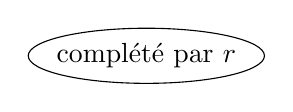
\begin{tikzpicture}\node at (0,0) {\unsure{complété par $r$}};\draw (0,0) ellipse (1.5 and .35);\end{tikzpicture}}
\figure{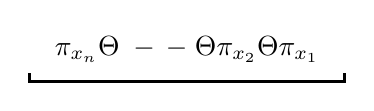
\begin{tikzpicture}
\node at (2,0.4) {$\pi_{x_n}\Theta\;-\,-\;\Theta\pi_{x_2}\Theta\pi_{x_1}$};
\draw[line width=1.3pt] (0,0.1)--(0,0)--(4,0)--(4,0.1);
\end{tikzpicture}}
\[p\supset q\supset r\]
\diagram{\begin{tikzcd}[ampersand replacement=\&]
A_{[p,q]}\\
A_q\arrow[u,"\text{local plat dim relative 0}"]
\end{tikzcd}}
\[ A_q/qA_q \]
\margin{\unsure{il y a donc un} \unsure{corps|anneau} \unsure{noethérien|non commutatif} de dim 1, savoir $A/q$, \unsure{dont on prend le complété} $-\ -\ -\ -\ -\ -$}
\[p\supset q\supset r\]
\figure{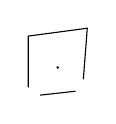
\begin{tikzpicture}[scale=.5]
\draw (0,0)--(0,1.3)--(1.5,1.5)--(1.4,.2);\draw (.3,-.2)--(1.2,-.1);\fill (.75,.5) circle (.035);
\end{tikzpicture}}
\diagram{\begin{tikzcd}[ampersand replacement=\&]
\widehat A_p\\ A_p\arrow[u]
\end{tikzcd}}
\[
A_{[p,q]}\otimes_{A_q} A_{\deleted{\unsure{p}}r}/r^n A_r
\]
\[
\underbrace{A_{[p,q]}/r^n A_{[p,q]}}_{\text{dim 1}}\otimes A_r\deleted{\unsure{A_q}}
\]
\unsure{complété de}
\[A/\]
\diagram{\begin{tikzcd}[ampersand replacement=\&,column sep=small]
A_{[p_1,\ldots,p_{n-1}]}\arrow[rr,"\deleted{\unsure{R}}"]\&\& A_{[p_1,-\,-\,;p_n]}\\
\&\deleted{A_{[p_1}}\arrow[ur]\&\\
\&\widehat A_{p_1}\arrow[r,dash]\&\widehat A_{p_i}\arrow[uu,no head,bend right=10]\arrow[r,dash]\&\widehat A_{p_n}\arrow[uul]
\end{tikzcd}}
\[A_{[p_1,\ldots,}\]
\figure{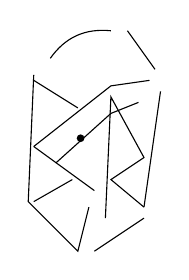
\begin{tikzpicture}[scale=.7]
\draw (0,2.8)--(-.1,.5)--(.8,-.4)--(1,.4);
\draw (.3,3.1) to[bend left] (1.4,3.6);\draw (1.7,3.6)--(2.2,2.9);
\draw (2.3,2.5)--(2,.4);\draw (1.1,-.4)--(2,.2);
\draw (0,2.7)--(.8,2.2);\draw (0,1.5)--(1.1,.7);\draw (0,.5)--(.7,.9);
\draw (0,1.5)--(1.4,2.6)--(2.1,2.7);\draw (.4,1.2)--(1.4,2.1)--(1.9,2.3);
\draw (1.3,.2)--(1.4,2.4)--(2,1.3)--(1.4,.9)--(2,.4);
\fill (.85,1.65) circle (.07);
\end{tikzpicture}}
\diagram{\begin{tikzcd}[ampersand replacement=\&]
\&\unsure{\mathcal C|C}\arrow[d]\&\\
{}\&\unsure{\text{Ch. Sat}|\text{An. Sat}}\arrow[l,dash dot,bend left=20]\&
\end{tikzcd}}
\figure{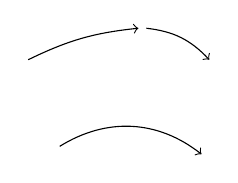
\begin{tikzpicture}
\draw[->] (0,1.2) to[bend left=10] (1.4,1.6);\draw[->] (1.5,1.6) to[bend left=20] (2.3,1.2);
\draw[->] (.4,.1) to[bend left=35] (2.2,0);
\end{tikzpicture}}
\diagram{\begin{tikzcd}[ampersand replacement=\&]
x_0\arrow[r,"\text{chaine saturée}"']\&x_n
\end{tikzcd}}
% archive sheet number: 61

\figure{\begin{tikzpicture}\draw (0,.25) to[out=-60,in=90] (.07,0);\end{tikzpicture}}
\scanpage{63}
\figure{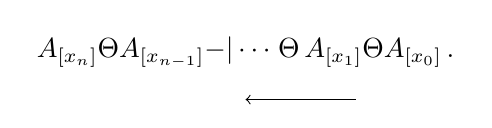
\begin{tikzpicture}
\node at (2,0.6) {$A_{[x_n]}\Theta A_{[x_{n-1}]}\unsure{\mathord{-}|\cdots}\;\unsure{\Theta}\, A_{[x_1]}\Theta A_{[x_0]}\,.$};
\draw[->] (3.4,0)--(2,0);
\end{tikzpicture}}
\figure{\begin{tikzpicture}
\draw (0,1.6)--(2,1.6);\foreach \x in {0,.4,1.6,2} \draw (\x,1.5)--(\x,1.7);
\draw[->,line width=1.2pt] (0,.8)--(1,.8);\draw[dashed] (1,.8)--(1.7,.8);\draw (0,.7)--(0,.9);\draw (1.7,.7)--(1.7,.9);
\draw (0,0)--(1.1,0);\draw[->,thick] (-.6,0)--(0,0);\draw (-.7,-.1)--(-.7,.1);\draw (0,-.1)--(0,.1);\draw (1.1,-.1)--(1.1,.1);
\end{tikzpicture}}
\figure{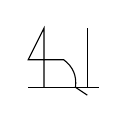
\begin{tikzpicture}[scale=.5]
\draw (0,0)--(1.8,0);\draw (.4,0)--(.4,1.5)--(0,.7)--(.9,.7) to[bend left] (1.2,0)--(1.5,-.2);\draw (1.5,0)--(1.5,1.5);
\end{tikzpicture}}
\diagram{\begin{tikzcd}[ampersand replacement=\&]
K_c\arrow[r]\&\prod_{c'}K_{c'}
\end{tikzcd}}
\[\operatorname{Hom}(K_{\unsure{*|\#}},K_{\unsure{*|\#}})\]
\[H_I(DD(A))=\underline{\unsure{\mathcal H|H}}^{**}(A)\]
\[A_x\]
\figure{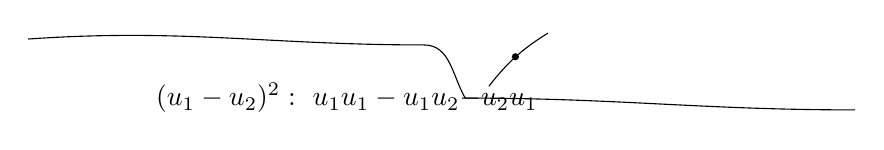
\begin{tikzpicture}[x=.75cm,y=.75cm]
\node[anchor=west] at (2,.1) {$(u_1-u_2)^2:\ u_1u_1-u_1u_2\unsure{-u_2u_1}$};
\draw (0,1.1) to[out=4,in=180] (6.7,1) to[out=0,in=120] (7.4,.1) to[out=0,in=180] (14,-.1);
\draw (7.8,.3) to[bend left=10] (8.8,1.2);\fill (8.25,.8) circle (.06);
\end{tikzpicture}}
\[\sum 1_{x_0,x_1}\qquad u_1\]
\diagram{\begin{tikzcd}[ampersand replacement=\&]
A_{c'}\times A_c\arrow[r]\&A_{c'c}
\end{tikzcd}}
si \uline{$c'$ et $c$} \uuline{\unsure{composables}} (\unsure{en cet ordre})
\figure{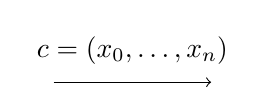
\begin{tikzpicture}
\node at (2,.4) {$c=(x_0,\ldots,x_n)$};\draw[->] (1,0)--(3,0);
\end{tikzpicture}}
\[c'=(x_n,\unsure{\ldots|x_{n+1}},x_m)\]
\[\unsure{v|u}\mathord{-}\]
\diagram{\begin{tikzcd}[ampersand replacement=\&]
A_{c'}\arrow[r,dash]\&A_{c'c}\\
A_c\arrow[r,dash]\&A_{c'c}
\end{tikzcd}}
\uline{Sinon on prend 0}

\deleted{\unsure{Évidemment}}
\diagram{\begin{tikzcd}[ampersand replacement=\&]
A_{c''}\times A_{c'}\times A_c\arrow[r]\arrow[d]\&A_{c''c'}\times A_c\arrow[d]\\
A_{c''}\unsure{\times}A_{c'c}\arrow[r]\&A_{c''c'c}
\end{tikzcd}}
\[\deleted{\unsure{*}}\]
\diagram{\begin{tikzcd}[ampersand replacement=\&,row sep=large]
\unsure{f,g,h|fg,h}\arrow[r]\&\bigl(\underbrace{i_{c'',c''c'}(f)i_{c',c''c'}(g)},\ h\bigr)\arrow[d]\\
\&\underbrace{i_{\unsure{c''c'},c''c'c}(\underline{\hspace{1cm}})}i_{\unsure{c},c''c'c}(h)
\end{tikzcd}}
\[i_{c'',c''c'c}(f)\ i_{c',c''c'c}(g)\ i_{c,c''c'c}(h)\]
\figure{\begin{tikzpicture}
\draw[->,thick] (0,0)--(1.2,0);\draw (0,-.1)--(0,.1);\node at (.6,.4) {$c$};
\draw[->,very thick] (1.6,0)--(2.9,0);\draw (1.6,-.1)--(1.6,.1);\node at (2.2,.4) {$c'$};
\draw (3.5,0)--(4.7,0);\draw[very thick] (4.7,-.1)--(4.7,.1);\node at (4.1,.4) {$c''$};
\node at (6,0) {$A_c$};
\end{tikzpicture}}
% archive sheet number: 62
